% !TEX root = ../chem_ia.tex
\section{Results}

\subsection{Raw Data}

\begin{table}[!htb]
\begin{minipage}[t]{.65\linewidth}
	\centering
	\begin{tabular}{|c|c|c|c|c|c|c|c|c|} 
		 \hline
		 \multirow{2}{*}{Setup} & \multicolumn{5}{c|}{Volumes $(\pm .05 mL)$} & \multicolumn{3}{c|}{Time $(\pm .05 s)$}\\
		 \cline{2-9}
		 & $HCl$ & $Acetone$ & $I_2$ & $H_2O$ & Total & $\#1$ & $\#2$ & $\#3$ \\
		  \hline
		 $\#1$ & $5$ & $5$ & $5$ & $10$ & $25$ & $342$ & $354$ & $331$\\
		  \hline
		  $\#2$ & $5$ & $5$ & $10$ & $5$ & $25$ & $621$ & $682$ & $634$\\
		  \hline
		  $\#3$ & $5$ & $10$ & $5$ & $5$ & $25$ & $161$ & $183$ & $164$\\
		  \hline
		  $\#4$ & $10$ & $5$ & $5$ & $5$ & $25$ & $152$ & $165$ & $153$\\
		  \hline
		\end{tabular}
		\caption{Rate Law Experiment (all trials performed at $294.8$ $K$)}
	\label{table:rate_law_raw_data}
    \end{minipage}%
\begin{minipage}[t]{.35\linewidth}
\centering
	\begin{tabular}{|c|c|c|c|} 
		 \hline
		 Temperature & \multicolumn{3}{c|}{Time $(\pm .05 s)$}\\
		 \cline{2-4}
		 $(\pm .05 K)$ & $\#1$ & $\#2$ & $\#3$ \\
		  \hline
		  $287.1$ & $734$ & $725$ & $756$\\
		  \hline
		  $294.8$ & $342$ & $354$ & $331$\\
		  \hline
		  $306.8$ & $134$ & $142$ & $115$\\
		  \hline
		  $317.5$ & $37$ & $42$ & $46$\\
		  \hline
		\end{tabular}
	\caption{Activation Energy Experiment (all trials carried out with volume setup $\#1$ in \cref{table:rate_law_raw_data})}
	\label{table:activation_energy_raw_data}
	\end{minipage}%
	\caption{Raw Data}
    \label{table:raw_data}
\end{table}

\subsection{Qualitative Data}
\begin{itemize}[itemsep=-1ex]
	  \item The iodine solution had a distinctive brownish-red color, similar to that of rust on iron metal.
	  \item A noticeable loss in color could be observed within the first $30$ seconds of the reaction, even for trials that took over $10$ minutes to come to full completion.
	  \item No observable immediate signs of a vigorous reaction could be observed (outside of the color loss) immediately after the addition of iodine to the remainder of the reactants.
	  \item The acetone had a relatively pungent odor similar to that of nail polish remover.
	  \item The iodine solution seemed to be particularly viscous, especially as opposed to the remainder of the reactants.
	\end{itemize}

\subsection{Calculations}

\subsubsection{Rate Law Experiment}

\begin{table}[H]
\centering

\begin{tabularx}{\textwidth}{|X|X|}
\hline 
 Rationale & Sample Calculation\\
 \hline
	Firstly, for each volumetric configuration, we must calculate the average time for the three unique trials performed, using the simple arithmetic mean formula:
	\[\bar{t}={\frac {1}{n}}\sum _{i=1}^{n}t_{i}\]
	where $n$ represents the number of trials ($3$).	
	& 
	Example for Setup $\# 1$: \newline

	{$\!\begin{aligned}
	\bar{t} &= \frac{(342 \pm .05) + (354 \pm .05) + (331 \pm .05)}{3} \\
	&= \frac{(1027 \pm .15)}{3} \\
	&= \SI{342 \pm .05}{\second}
	\end{aligned}$} \\
  \hline
Then, we must calculate the concentrations of each reactant based on the total volume and their specific volume using the mole-constant dilution formula:

\[M_1V_1 = M_2V_2 \textit{ or } M_2 = \frac{M_1V_1}{V_2} \]

where $M_1$ is the initial molarity of the reactant, $V_1$ is the initial volume of the reactant, and $V_2$ is the total volume ($25 mL$). We can additionally calculate potential discrepancies for the largest percent uncertainty and then propagate this error for the remaining results.
	& 
	Example for Setup $\# 1$: \newline

	{$\!\begin{aligned}
	\left[I_2\right] &= \frac{\SI{.005}{\molar} \times \SI{5 \pm .05}{\milli\liter}}{\SI{25 \pm .2}{\milli\liter}} = \frac{(.025 + .00025)}{(25 \pm .2)} \\
	&= \frac{(.025 + 1\%)}{(25 \pm .8\%)} = .001 \pm 1.8\% \\
	&= \SI{.001 \pm .000018}{\molar} 
	\end{aligned}$} 

Through an identical process, the final concentrations of $[HCl]$ and $[Acetone]$ can also be determined. Because $[I_2]$ has the smallest quantity, it has the largest percent error of $1.8\%$, which is carried over for all final concentrations. \\
\hline

Using the two above steps, we can then determine the rate for each individual configuration using the previously discussed equation:

\[rate = \frac{[I_2]}{\bar{t}}\]

The same propagation approach is utilized, but the uncertainties are largely irrelevant for the purpose of rate calculation which is predicated on approximation already.
&
Example for Setup $\# 1$: \newline

	{$\!\begin{aligned}
	rate &= \frac{\SI{.001 \pm .000018}{\molar}}{\SI{342 \pm .05}{\second}} \\
	&= \frac{.001 \pm 1.8\%}{342 \pm .01\%} = \num{2.92e-6} \pm 1.81\% \\
	&= \SI{2.92e-6}{\molar\per\second}
	\end{aligned}$} \\

  \hline
After determining the rates for all trials, we can compare the rates for configurations $2-4$ to the baseline provided by $1$ to determine the rate law. As in each of the last $3$ trials, the concentration of one reactant was changed while maintaining the total volume, the concentration of that reactant is doubled for that specific trial. Thus, we can calculate our order $m$ by the formula:

\[m = \log_2 \left(\frac{rate_i}{rate_1}\right)\]

where $rate_i$ is the rate for the given setup and $rate_1$ is the rate for configuration $\#1$. The result must be approximated, as $m$ must be a whole integer $>=0$.
&
Example for Setup $\# 4$ (compared to the baseline of Setup $\# 1$):

	\[m = \log_2 \left(\frac{\num{6.37e-6}}{\num{2.92e-6}}\right) = \log_2 2.18 = 1.12 \approx \bm{1}\]

Thus, the concentration of $HCl$ is first order with respect to the overall reaction based on this determination. The remaining orders are also calculated in the same manner. \\

\hline

\end{tabularx}
\caption{Rate Law Calculations}
\label{table:rate_law_calculations}
\end{table}

Using this process for all trials, the order of $HCl$, $Acetone$, and $I_2$ are found to be $1$, $1$, and $0$ respectively. This confirms the theorized rate law of $rate = k[HCl][CH_3COCH_3]$ and is further supported by the published literature on this subject~\parencite{main_literature}. Through this knowledge, we can now determine the activation energy.
\newpage
\subsubsection{Activation Energy Experiment}

\begin{table}[h!]
\centering

\begin{tabularx}{\textwidth}{|X|X|}
\hline 
 Rationale & Sample Calculation\\
 \hline
 \multicolumn{2}{|>{\hsize=\dimexpr2\hsize+2\tabcolsep+\arrayrulewidth\relax}X|}{The first three steps--calculating the average (mean) time for each temperature, determining diluted concentrations, and finding the rate using those two values--are identical for this section as well, and are thus not included to limit redundancy. \newline}
\\
\hline
After these three steps, we must determine the value of the rate constant $k$, which we can do by utilizing the rate law. As $rate = k[HCl][Acetone]$, we can rearrange to get:

\[k = \frac{rate}{[HCl][Acetone]}\]

Furthermore, the concentrations of $HCl$ and $Acetone$ are consistent for all temperatures as identical volumes were chosen to ease calculations and limit confounding variables.
&
Example for $\SI{294.8}{\kelvin}$: \newline

{$\!\begin{aligned}
	k &= \frac{(\num{2.92e-6} \pm 1.9\%)}{(.2 \pm 1.8\%) \times (.8 \pm 1.8\%)} \\
	&= \num{1.83e-5} \pm 5.5\% \\
	&= \SI{1.83\pm.10e-5}{\cubic\deci\metre\per\mol\per\second}
	\end{aligned}$}
\\
 \hline
 After determining $k$ at each temperature, we will create an Arrhenius graph to determine the activation energy. Taking the natural logarithm of the Arrhenius equation results in:

\[\ln{k} = \left(\frac{-E_a}{R}\right)\frac{1}{T} + \ln{A}\]

Thus, a linear relationship exists between $\ln{k}$ and $\frac{1}{T}$, so these values must be determined (along with their uncertainties) for the purpose of graphing.

&
Example for $\SI{294.8}{\kelvin}$: \newline

{$\!\begin{aligned}
	\frac{1}{T} &= \frac{1}{\SI{294.8 \pm .05}{\kelvin}} = \frac{1}{(294.8 \pm .017\%)} \\
	&=  .00339 \pm .017\% = \SI{3.39\pm.00058e-3}{\per\kelvin}
	\end{aligned}$} 

\rule{0pt}{3ex}   

{$\!\begin{aligned}
	\ln{k} &= \ln{\left(\num{1.83\pm.10e-5}\right)} = \ln{\left(\num{1.83e-5}\right)} + \frac{.10}{1.83} \\
	&= -10.91 \pm .05
	\end{aligned}$} \\

\hline
\end{tabularx}
\caption{Activation Energy Calculations}
\label{table:activation_energy_calculations}
\end{table}

This process is again carried out for all four temperatures, providing the necessary values for graphing purposes.

\subsection{Processed Data}

\begin{table}[!htb]
\centering
	\begin{tabular}{|c|c|c|c|} 
		 \hline
		 Setup & Avg. Time ($\pm \SI{.5}{\second}$) & Rate ($\si{\molar\per\second}$) \\
		 \hline
		  $\#1$ & $342$ & $\num{2.92\pm.053e-6}$\\
		  \hline
		  $\#2$ & $646$ & $\num{3.10\pm.056e-6}$\\
		  \hline
		  $\#3$ & $169$ & $\num{5.92\pm.107e-6}$\\
		  \hline
		  $\#4$ & $157$ & $\num{6.37\pm.115e-6}$ \\
		  \hline
		 \end{tabular}
		\caption{Rate Law Experiment (all trials performed at $\SI{294.8}{\kelvin}$)}
	\label{table:rate_law_processed_data}
\end{table}

\begin{table}[htb!]
\centering
	\begin{tabular}{|c|c|c|c|} 
		 \hline
		 Temperature & $k$ ($\si{\cubic\deci\metre\per\mol\per\second}$) & $\frac{1}{T}$ ($\pm .17\%$) ($\si{\per\kelvin}$) & $\ln{k}$ ($\pm .055$) \\
		  \hline
		  $287.1$ & $\num{8.47\pm.47e-6}$ & $\num{3.48e-3}$ & $-11.68$ \\
		  \hline
		  $294.8$ & $\num{1.83\pm.10e-5}$ & $\num{3.39e-3}$ & $-10.91$\\
		  \hline
		  $306.8$ & $\num{4.81\pm.26e-5}$ & $\num{3.26e-3}$ & $-9.94$\\
		  \hline
		  $317.5$ & $\num{1.49\pm.08e-4}$ & $\num{3.15e-3}$ & $-8.81$\\
		  \hline
		\end{tabular}
	\caption{Activation Energy Experiment (all trials carried out with volume setup $\#1$ in \cref{table:rate_law_raw_data})}
	\label{table:activation_energy_processed_data}
\end{table}

As determined already, the rates in the Rate Law Experiment were sufficient for calculating/deriving the rate law of the overall reaction. However, to calculate the activation energy, the values of $\ln{k}$ and $\frac{1}{T}$ were plotted and a linear regression was utilized to calculate a line of best fit (to allow for the determination of the gradient between the 2 variables). The table, including data points and uncertainties, are depicted in \cref{fig:arrhenius}. The initial best fit line (for the entire dataset) had a very high correlation coefficient ($R^2$) of around $99\%$, indicating a good fit, however this value was partially misleading. By significantly overshooting the data point at $\SI{294.8}{\kelvin}$, the regression was able to overcome its slightly lower predictions at the other three temperatures. In fact, this line of best fit was completely outside of the range of uncertainty for the data point at $\SI{287.1}{\kelvin}$. By removing the outlier at $\SI{294.8}{\kelvin}$, a new trend line was produced with a $R^2$ of $99.5\%$ and a much better ability to account for the actual data points. However, both lines seemed to generate similar gradients, thus minimizing the overall impact of the improved regression.

To determine the uncertainty of the coefficients in the regression, the statistical premise of $95\%$ confidence intervals was employed. Using the $\frac{1}{T}$ as the $x$ variable and the $\ln{k}$ as the $y$, the following procedure was used for the regression of $y = \beta x + \alpha$~\parencite{regression_stat_book}.

 \begin{minipage}{.5\linewidth}
  $$S_x = \sum x_i = 13.28$$
  $$S_y = \sum y_i = -41.34$$
  $$S_{xx} = \sum x_i^2 = 44.15$$
  $$S_{yy} = \sum y_i^2 = 431.87$$
  $$S_{xy} = \sum x_iy_i = -137.79$$
 \end{minipage}
  \begin{minipage}{.5\linewidth}
  $$\hat{\beta} = \frac{nS_{xy} - S_xS_y}{nS_{xx} - S_x^2} = -8.54$$
  $$\hat{\alpha} = \frac{1}{n}S_y - \hat{\beta}\frac{1}{n}S_x =  18.02$$
  $$s_{\epsilon}^2 = \frac{1}{n(n-2)}\left[nS_{yy} - S_y^2 - \hat{\beta}^2(nS_{xx} - S_x^2)\right] = .01005$$
  $$s_{\hat{\beta}}^2 = \frac{ns_{\epsilon}^2}{nS_{xx} - S_x^2} = .160$$
  $$\beta \in [\hat{\beta} \mp t_{2}^*s_{\hat{\beta}}] = \bm{-8.54} \bm{\pm} \bm{1.72}$$
 \end{minipage}

 Thus, the gradient ($\beta$) is $-8.54 \pm 1.72$, which can be equated to the slope of the relationship in the Arrhenius equation ($\frac{-E_a}{R}$) to determine the activation energy (using the universal gas constant $R$). The factor of $10^3$ is also reincorporated, as the inverse temperature values had been normalized by factoring out $10^{-3}$ for improved graphing:

 \[E_a = \SI{-8.54\pm1.72}{\per\kelvin} \times -\SI{8.3145}{\joule\per\mole\per\kelvin} \times 10^3 = (-8.54 \pm 20.1\%) \times -8.3145 \times 10^3 = 71005.83 \pm 20.1\% = \SI{71.01\pm14.27}{\kilo\joule\per\mole}\]

 Using the literature value of $\SI{86.60}{\kilo\joule\per\mole}$, the percent error can also be determined:

 \[\textit{Total Percent Error} = \left|\frac{\textit{Literature Value - Experimental Value}}{\textit{Literature Value}}\right| \times 100 = \left|\frac{\textit{86.60 - 71.01}}{\textit{86.60}}\right| \times 100 = 18.0\%\]



% !TEX root = ../chem_ia.tex
\begin{figure}[!htb]
    \centering
    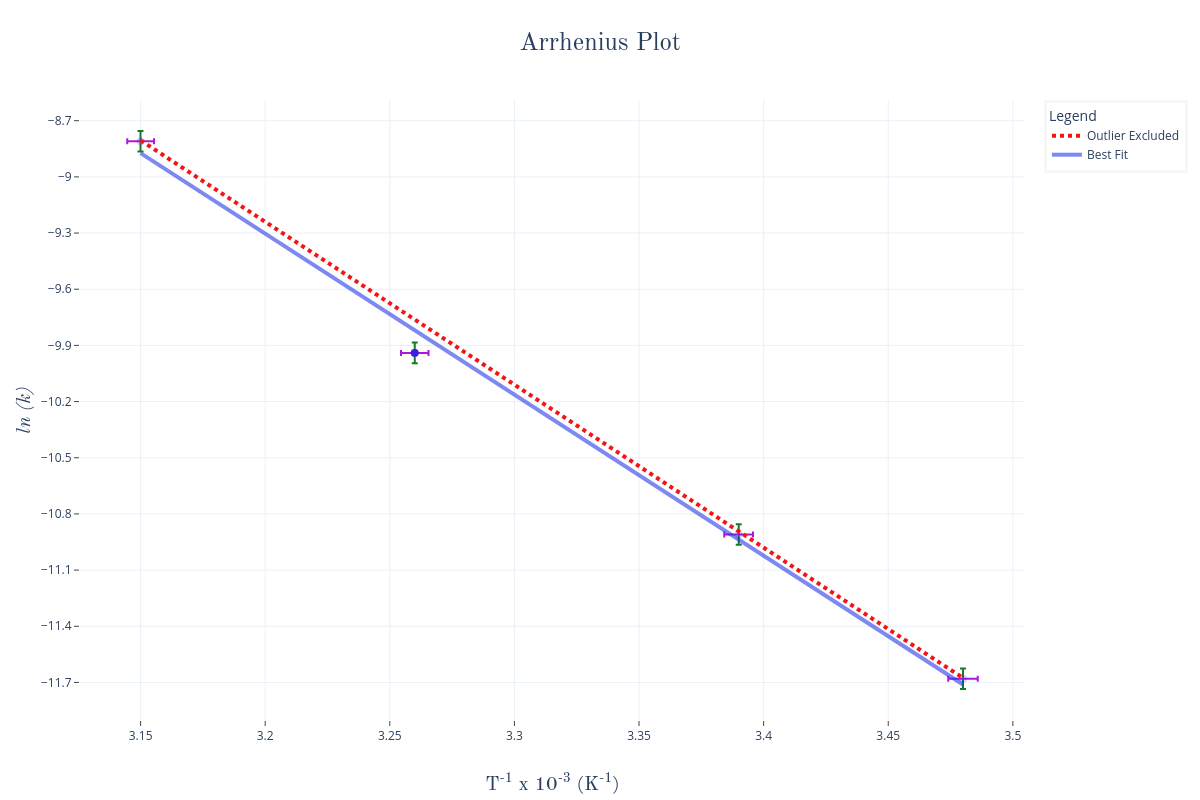
\includegraphics[width=1.0\textwidth]{fig/images/arrhenius.png}
    \caption{Arrhenius plot of $\ln{k}$ versus $\frac{1}{T}$ (scaled by $10^3$), including a best fit line for the general data and an improved trendline with the outlier removed.}
    \label{fig:arrhenius}
\end{figure}

\subsection{Analysis}
Overall, there do not appear to be any serious/obvious anomalies for all data collected in this experiment. The general trend line depicted in the linear regression of \cref{fig:arrhenius} is consistent with the scientific theory of the Arrhenius Equation and the linear relationship between the natural log of the rate constant and the inverse of the temperature of the reaction. The data collected for the trial at $\SI{294.8}{\kelvin}$ did appear to be an anomaly based on this statistical regression, however it was used to accurately determine the rate law for the overall stoichiometric reaction and its elimination did not result in a significantly larger correlation coefficient, indicating that it may not be as large of a structural deviation as initially thought. One possible explanation for this, however, may be that there were major fluctuations in room temperature at the time of the experiment, leading to a consistent change in proportions for all data calculated during thos trials. This explanation would account for the correct rate law being empirically derived from data at this temperature, and would also explain the reason for its status as an apparent outlier in the multi-temperature regression. The high $R^2$ value also suggests a strong statistical significance of the determined results, further providing support to the initial claims and lending credibility to the design and implementation of the experiment in its entirety. The uncertainties of the results were generally low for the majority of measurements, including those for temperature and volume, however the error for the final regression (and thus the activation energy) did become large due to a limited dataset size. This large error indicates systematic errors in the premise of the experiment, which will be further analyzed. 
